% Created 2021-09-27 Mon 11:53
% Intended LaTeX compiler: xelatex
\documentclass[letterpaper]{article}
\usepackage{graphicx}
\usepackage{grffile}
\usepackage{longtable}
\usepackage{wrapfig}
\usepackage{rotating}
\usepackage[normalem]{ulem}
\usepackage{amsmath}
\usepackage{textcomp}
\usepackage{amssymb}
\usepackage{capt-of}
\usepackage{hyperref}
\setlength{\parindent}{0pt}
\usepackage[margin=1in]{geometry}
\usepackage{fontspec}
\usepackage{svg}
\usepackage{cancel}
\usepackage{indentfirst}
\setmainfont[ItalicFont = LiberationSans-Italic, BoldFont = LiberationSans-Bold, BoldItalicFont = LiberationSans-BoldItalic]{LiberationSans}
\newfontfamily\NHLight[ItalicFont = LiberationSansNarrow-Italic, BoldFont       = LiberationSansNarrow-Bold, BoldItalicFont = LiberationSansNarrow-BoldItalic]{LiberationSansNarrow}
\newcommand\textrmlf[1]{{\NHLight#1}}
\newcommand\textitlf[1]{{\NHLight\itshape#1}}
\let\textbflf\textrm
\newcommand\textulf[1]{{\NHLight\bfseries#1}}
\newcommand\textuitlf[1]{{\NHLight\bfseries\itshape#1}}
\usepackage{fancyhdr}
\pagestyle{fancy}
\usepackage{titlesec}
\usepackage{titling}
\makeatletter
\lhead{\textbf{\@title}}
\makeatother
\rhead{\textrmlf{Compiled} \today}
\lfoot{\theauthor\ \textbullet \ \textbf{2021-2022}}
\cfoot{}
\rfoot{\textrmlf{Page} \thepage}
\renewcommand{\tableofcontents}{}
\titleformat{\section} {\Large} {\textrmlf{\thesection} {|}} {0.3em} {\textbf}
\titleformat{\subsection} {\large} {\textrmlf{\thesubsection} {|}} {0.2em} {\textbf}
\titleformat{\subsubsection} {\large} {\textrmlf{\thesubsubsection} {|}} {0.1em} {\textbf}
\setlength{\parskip}{0.45em}
\renewcommand\maketitle{}
\author{Taproot}
\date{\today}
\title{Handout 19 responses: fundamental theorem of calculus}
\hypersetup{
 pdfauthor={Taproot},
 pdftitle={Handout 19 responses: fundamental theorem of calculus},
 pdfkeywords={},
 pdfsubject={},
 pdfcreator={Emacs 28.0.50 (Org mode 9.4.4)}, 
 pdflang={English}}
\begin{document}

\tableofcontents

\section{Let \(F(x) = \int_{0}^{x} f(t) dt\)}
\label{sec:org5110d9d}
\subsection{complete the table}
\label{sec:org8cb3a14}
\begin{center}
\begin{tabular}{lrrrrr}
x & 0 & 1 & 2 & 3 & 4\\
F(x) & \(0\) & \(\frac{4}{3}\) & \(\frac{8}{3}\) & \(\frac{4}{3}\) & \(0\)\\
\end{tabular}
\end{center}

\subsection{sketch the function}
\label{sec:orgf412cf8}
\begin{center}
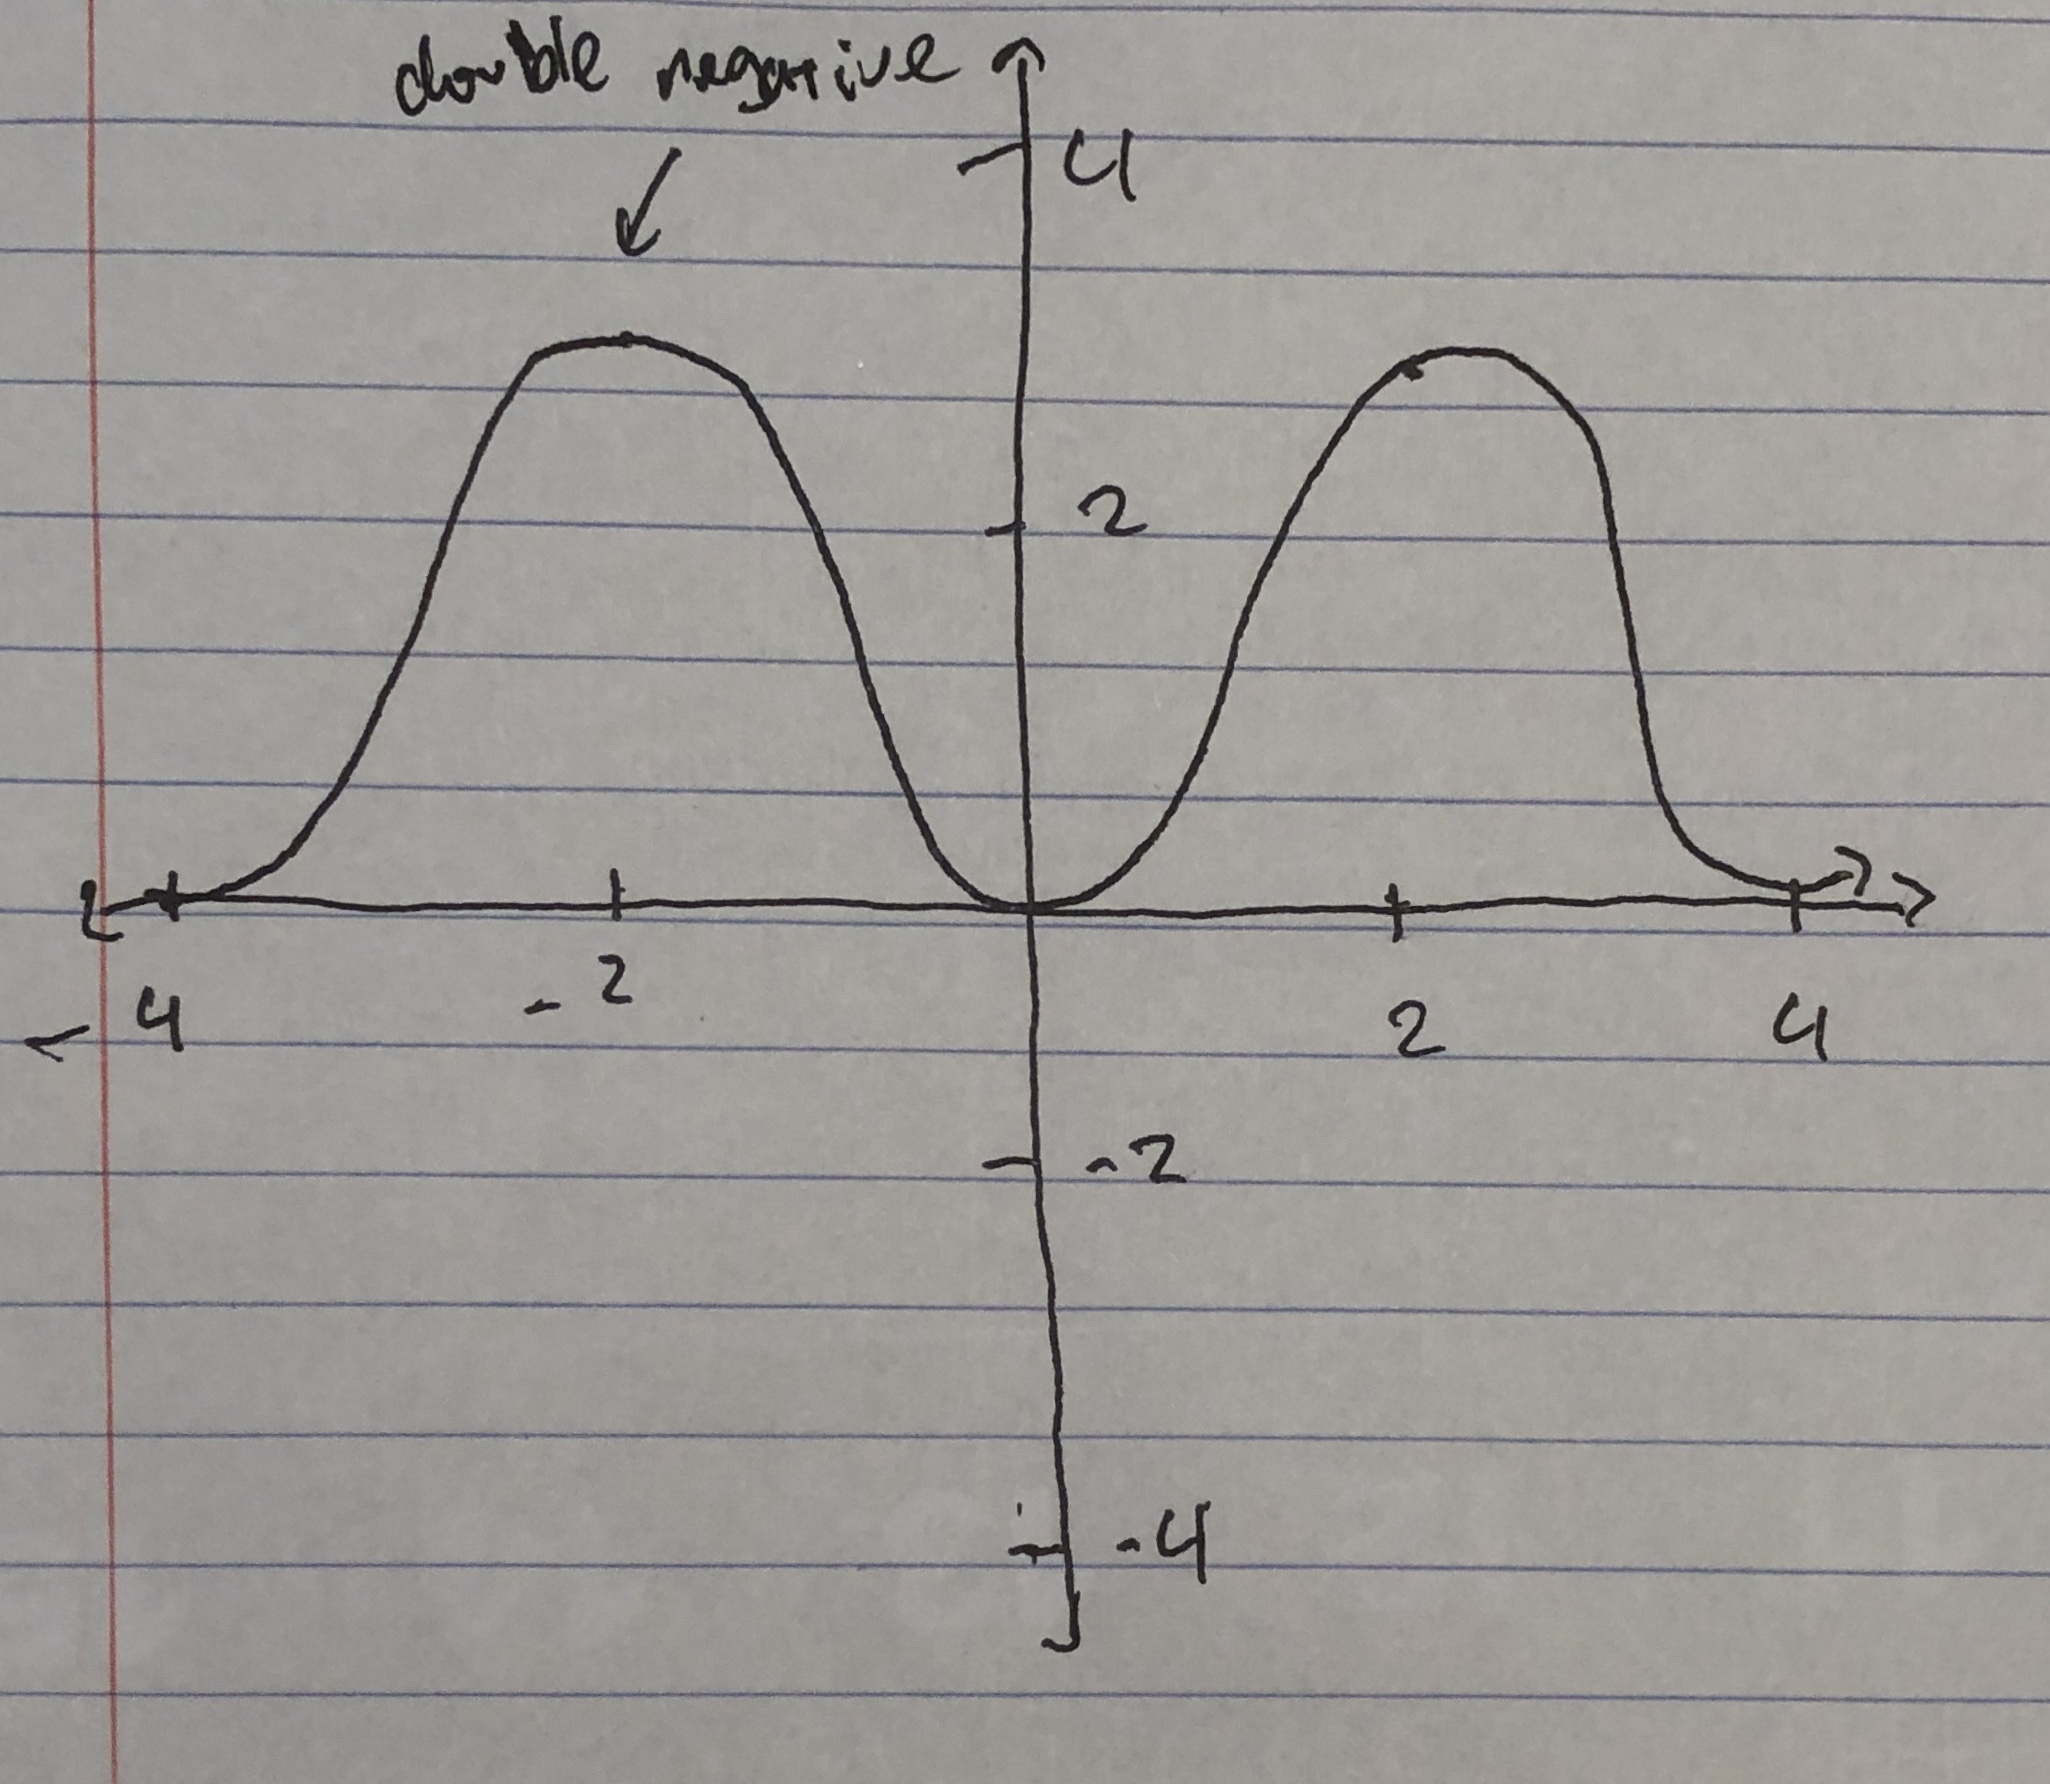
\includegraphics[width=.9\linewidth]{KBe21math401ret19src1b.png}
\end{center}

\section{\(G(x) = \int_{2}^{x} f(t) dt\)}
\label{sec:org2d86a55}

\subsection{complete the table}
\label{sec:orgac756f4}
\begin{center}
\begin{tabular}{lrrrrr}
x & 0 & 1 & 2 & 3 & 4\\
G(x) & \(-\frac{8}{3}\) & \(-\frac{4}{3}\) & \(0\) & -\(\frac{4}{3}\) & \(-\frac{8}{3}\)\\
\end{tabular}
\end{center}


\subsection{sketch the function}
\label{sec:org9b0e71a}
\begin{center}
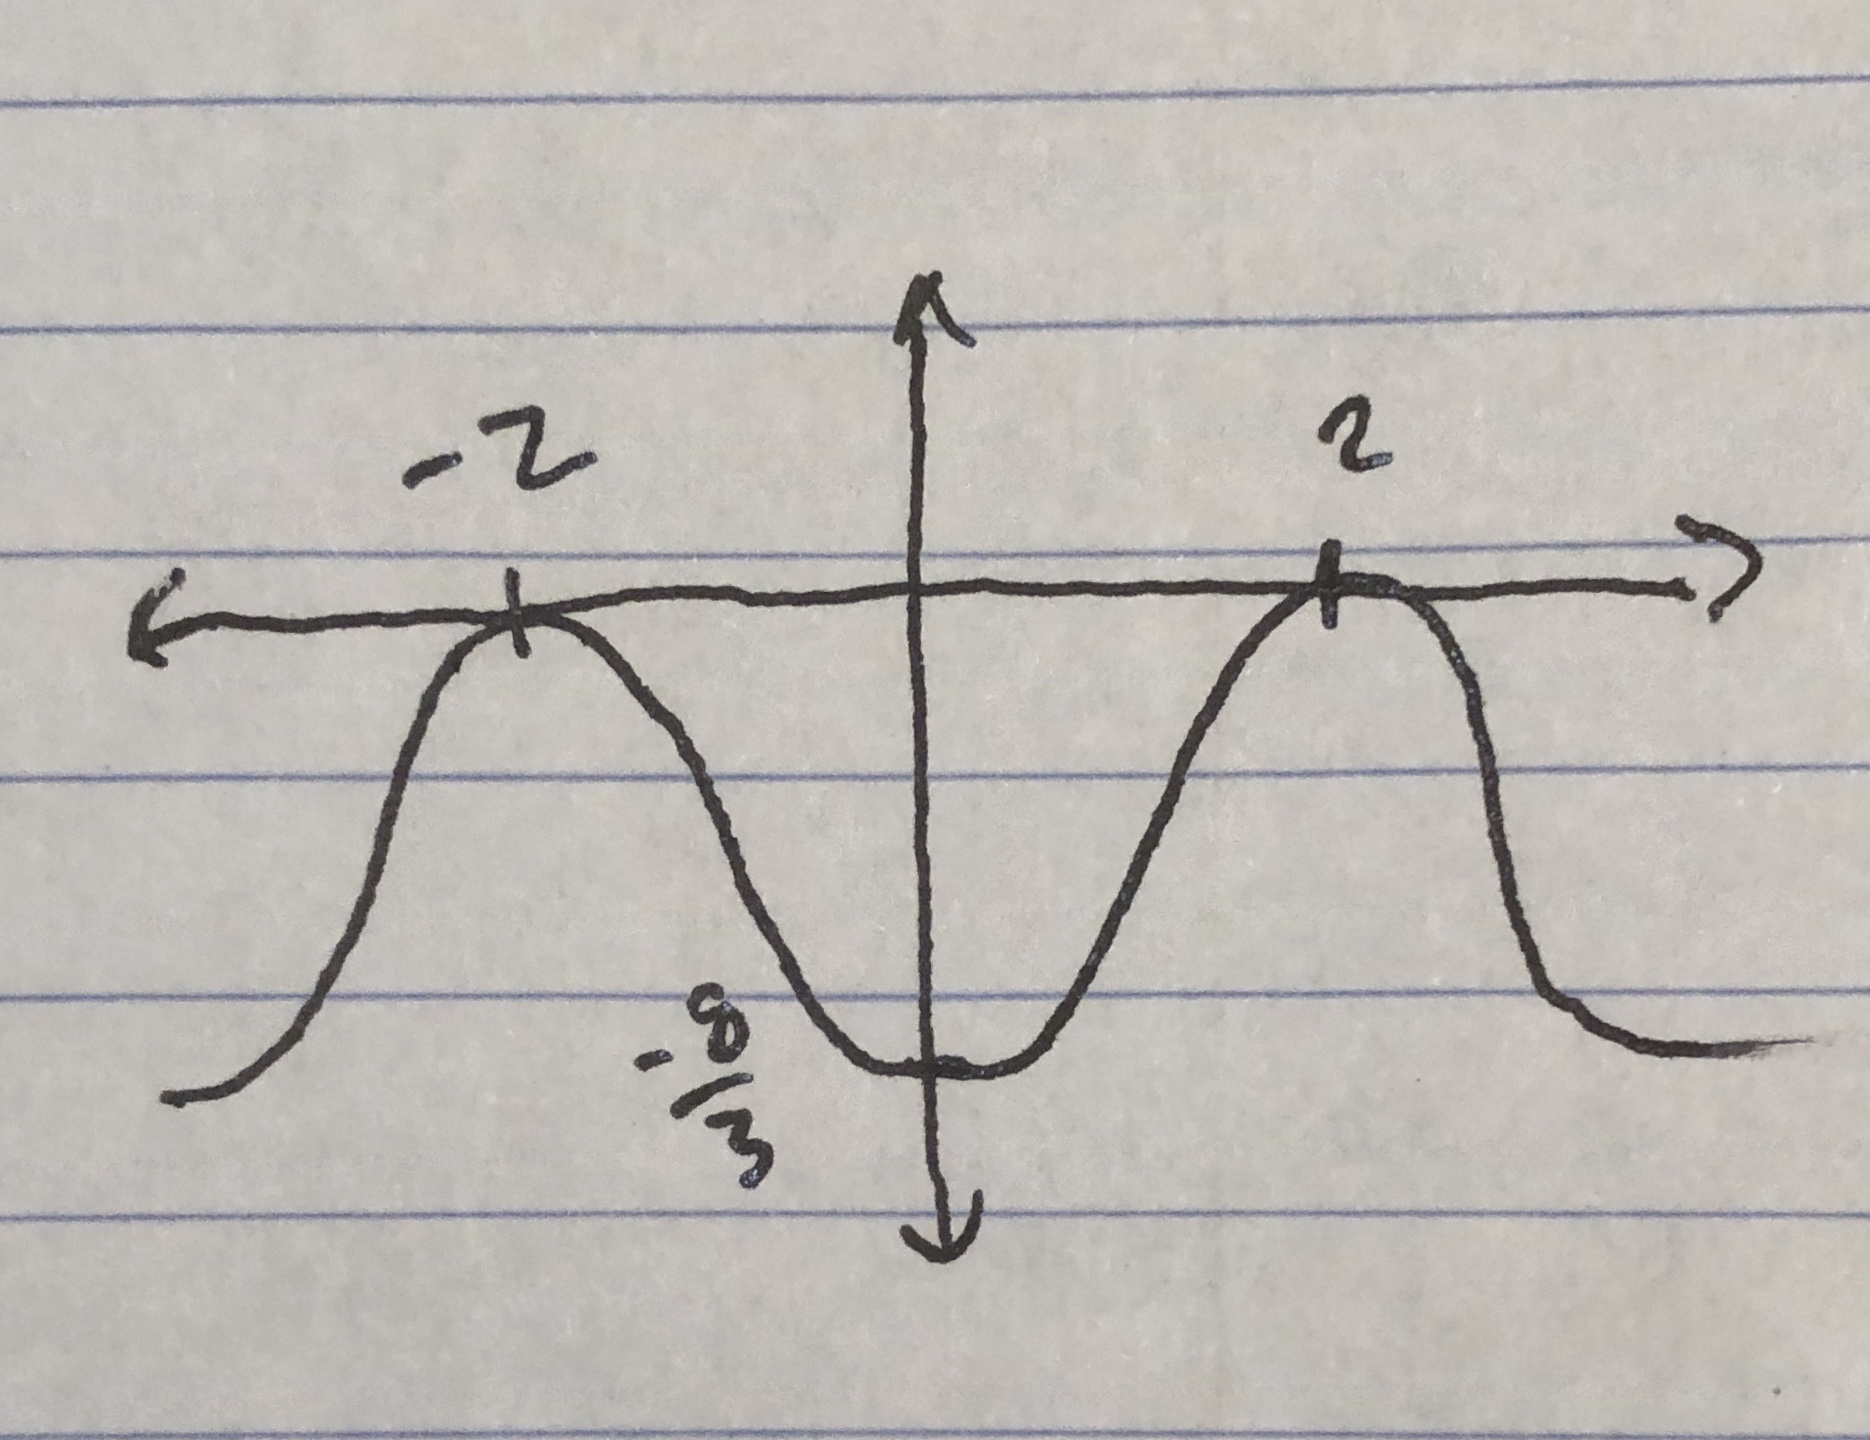
\includegraphics[width=.9\linewidth]{KBe21math401ret19src2b.png}
\end{center}

\section{\(H(x) = \int_4^x f(t) dt\)}
\label{sec:org2b7c86f}

\subsection{complete the table}
\label{sec:org8fbea2d}
\begin{center}
\begin{tabular}{lrrrrr}
x & 0 & 1 & 2 & 3 & 4\\
H(x) & \(0\) & \(\frac{4}{3}\) & \(\frac{8}{3}\) & \(\frac{4}{3}\) & \(0\)\\
\end{tabular}
\end{center}

\subsection{sketch the function}
\label{sec:org71f1c23}
same as 1b

\section{complete the table}
\label{sec:org7174c7e}
\begin{center}
\begin{tabular}{llll}
 & \(F(x)\) & \(G(x)\) & \(H(x)\)\\
maximum & 4n+2 &  & \\
minimum & 4n &  & \\
increases & \[4n, 4n+2\] &  & \\
decreases & \[4n-2, 4n\] &  & \\
\end{tabular}
\end{center}
The other columns are the same, because \(H(x) = F(x)\) and \(G(x) = H(x)-\frac{8}{3}\).

\section{why does it work over the entire domain?}
\label{sec:orgb2a9c9b}
The argument for each cell is the same: it should work across the domain because those are the points where the derivative of \(F(x)\) (which is \(f(x)\)) is zero and function is periodic.

\(F(x)\) increases when \(f(x)\) is positive.

\section{family of functions}
\label{sec:org7488574}
Changing the 'zero point' of the derivative just shifts the graph up and down, by up to the range of the function.

\section{sketching more functions}
\label{sec:org910765a}

\subsection{\(F_1(x) = \int_{x}^{0} f(t) dt\)}
\label{sec:org59366a7}
\(F(x)\) but reflected across the x-axis (negated)

\subsection{\(F_2(x) = \int_{0}^{x} f(-t) dt\)}
\label{sec:org49efd24}
\(f\) is an odd function so \(f(-t) = -f(t)\) so \(F_2 = F_1\)

\subsection{\(F_3(x) = \int_{0}^{2x} f(t) dt\)}
\label{sec:org8d65251}
\(F_3(x) = F(2x)\) which is a parent function transformation which compresses the graph along the x-axis.

\subsection{\(F_4(x) = \int_{0}^{x} f(|t|) dt\)}
\label{sec:org8c06269}
For \(x \ge 0\), \(F_4(x) = F(x)\). However, for \(x < 0\), the function will be the negative of the \(x\geq 0\) case because the integral is from right to left.

\begin{center}
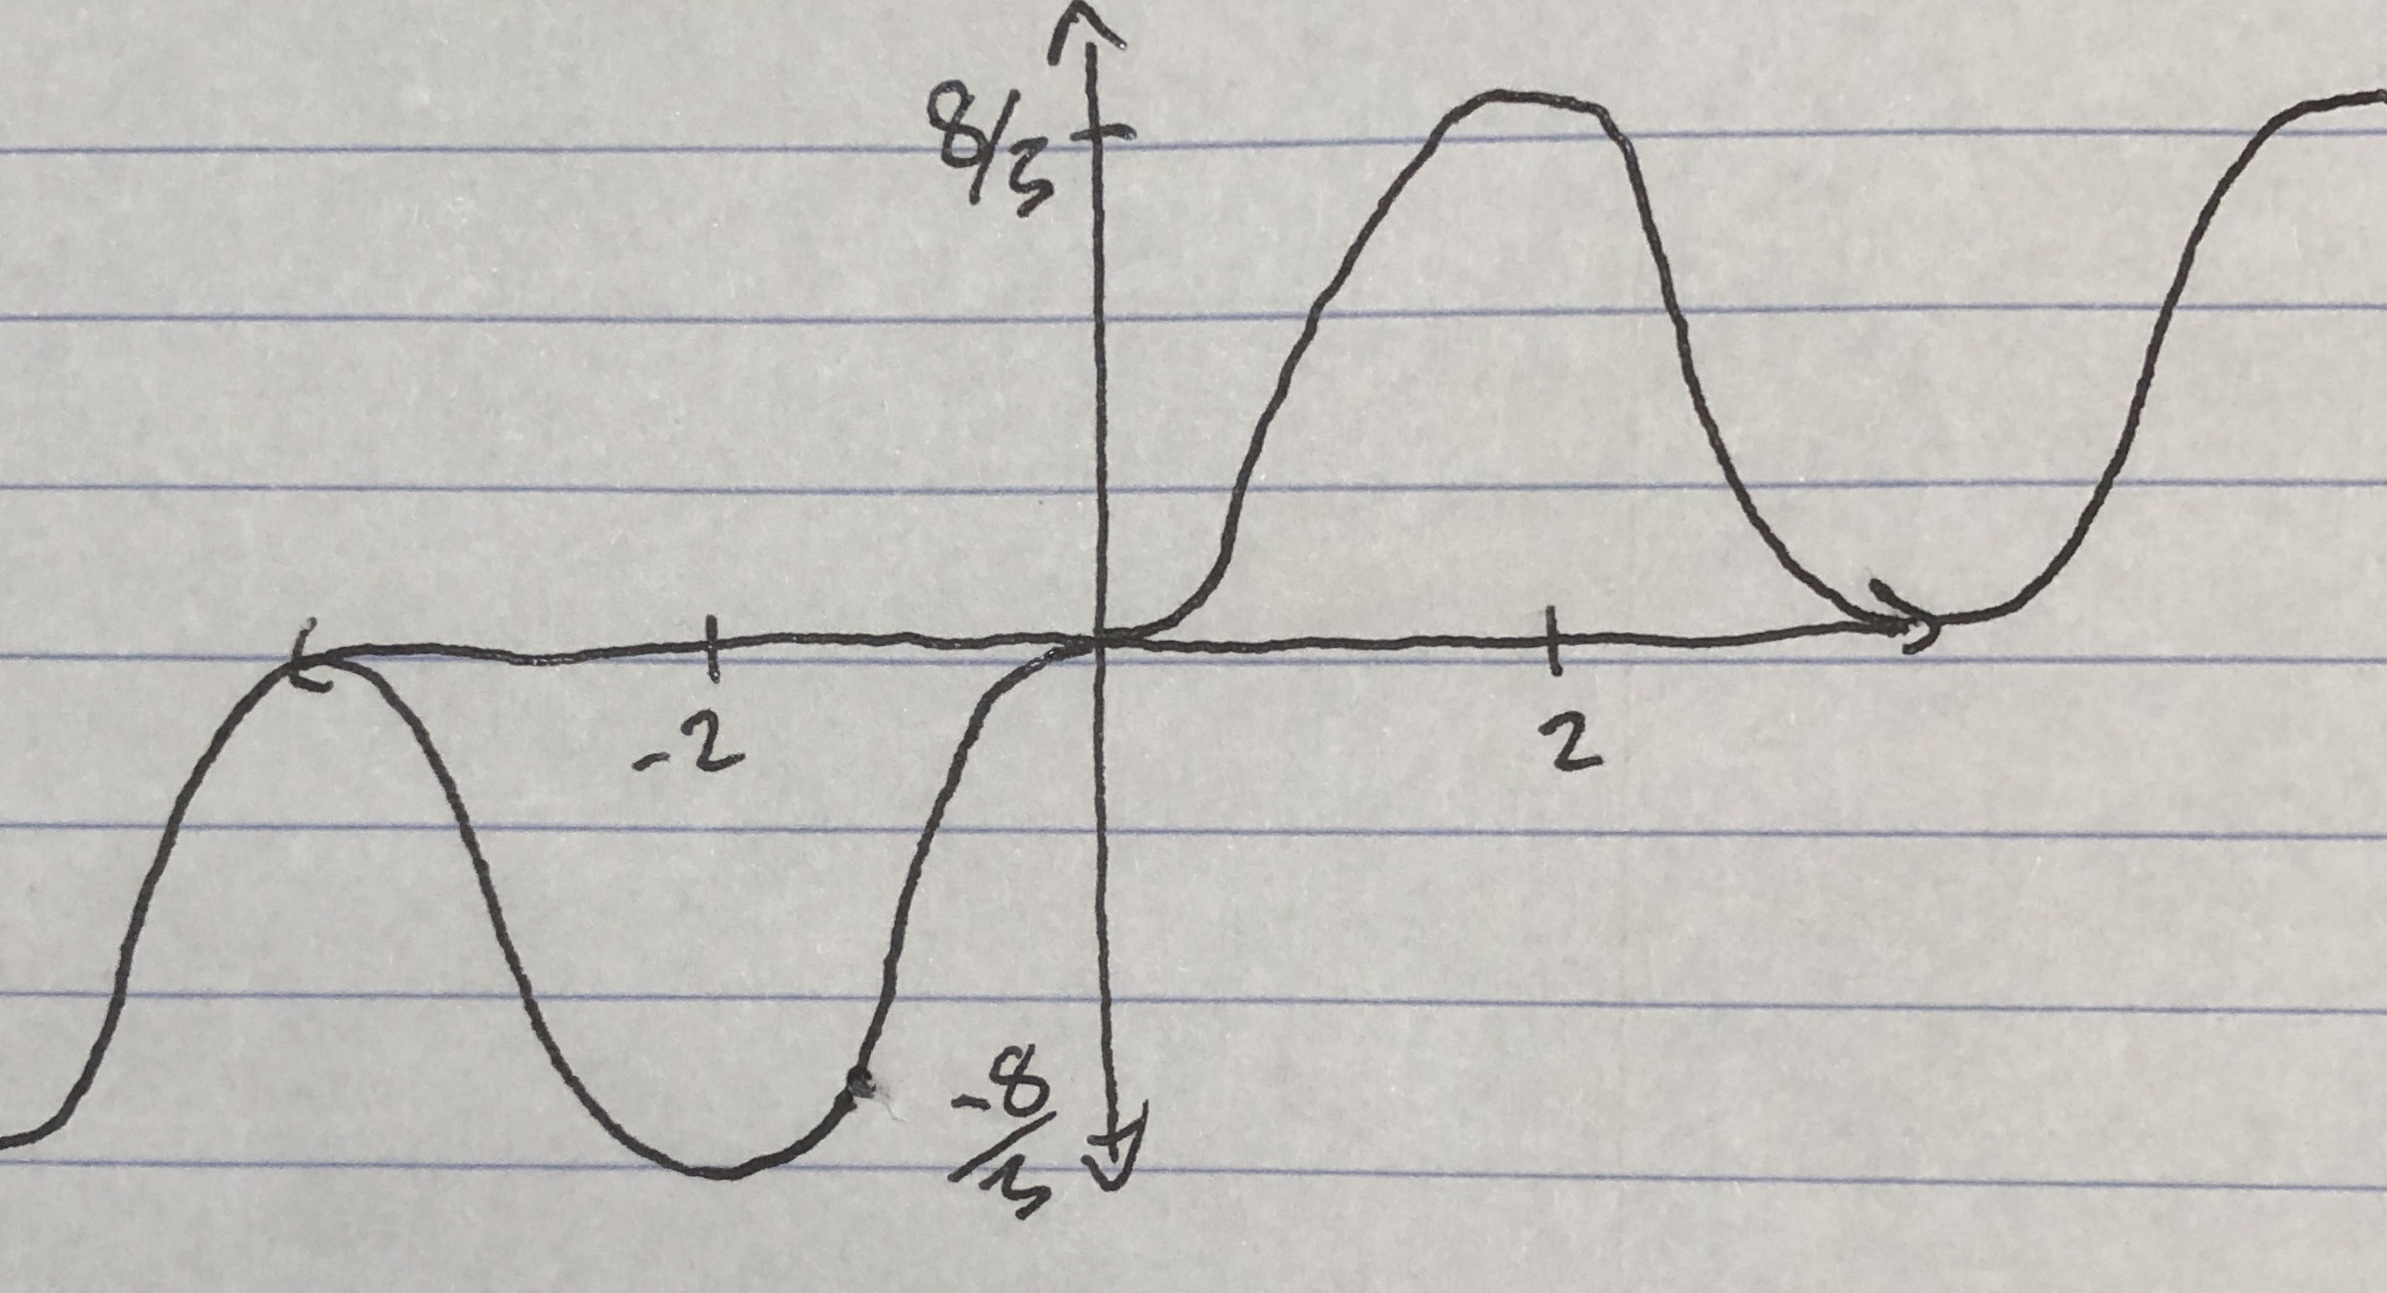
\includegraphics[width=.9\linewidth]{KBe21math401ret19src7d.png}
\end{center}

\subsection{\(F_5(x) = \int_{0}^{x} |f(t)| dt\)}
\label{sec:org0870c4e}
Instead of being a periodic function, this function will be even (all the decreasing parts of \(F(x)\) become increasing with the same shape)

\begin{center}
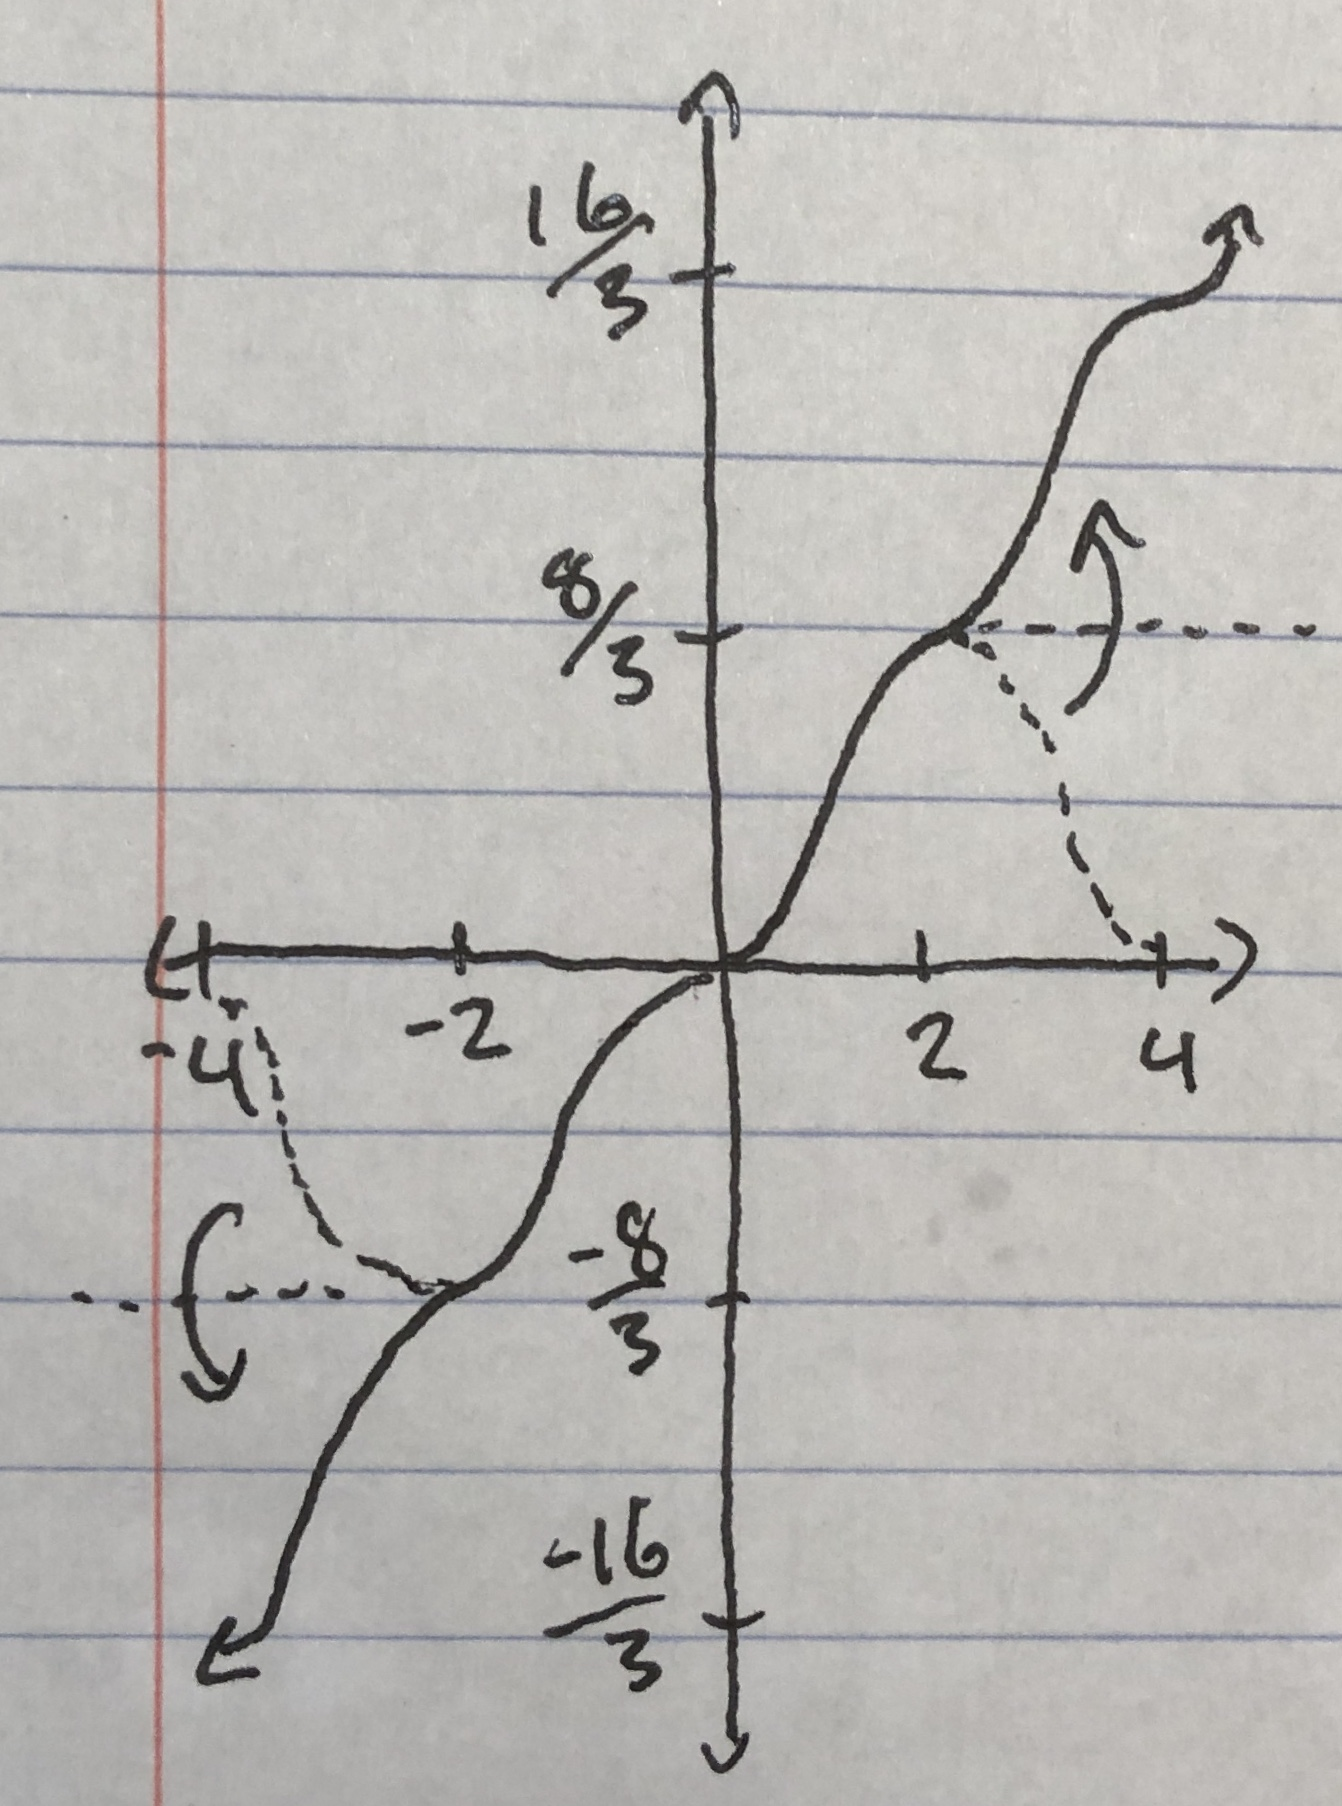
\includegraphics[width=.9\linewidth]{KBe21math401ret19src7e.png}
\end{center}


\section{derivatives of integral functions}
\label{sec:org52255bd}

\subsection{\(F(x) = \int_{-1}^{x^2} \sin(t^3-1) dt\)}
\label{sec:org1fbf028}

\[\begin{aligned}
   f(x) &= \int_{-1}^{x} \sin(t^3-1) dt\\
   F(x) &= f(x^2)\\
   \frac{d}{dx}F(x) &= \frac{d}{dx}f(x^2)\\
   &= f'(x^2)(2x)\\
   &= 2x \sin (x^{2^3}-1)
   \end{aligned}\]

\subsection{\(F(x) = \int_{0}^{2x} \ln(t-3) dt\)}
\label{sec:org2d3396d}

\[\begin{aligned}
   \frac{d}{dx}\left( \int_{0}^{2x} \ln(t-3) dt\right) &= 2 \frac{d}{dx}\int_{0}^{2x} \ln(t-3)dt\\
   &= 2 \ln(2x-3)
   \end{aligned}\]
\end{document}
